\section{Future Work}\label{future-work}

Ideally, our work would have resulted in a complete taxonomy of software
testing terminology based on the literature. Unfortunately, we were not able to
fully accomplish this due to time constraints. With more time, we would
continue iterating over undefined terms (\Cref{future-undef-terms}) and
investigate terms we \emph{expected} to find but never did
(\Cref{future-miss-terms}). Additionally, there is much more work we could do
to analyze our data on the software testing literature, such as detecting
more classes of flaws (and identifying them!) (\Cref{future-detect-flaws}).

\subsection{Iterating Over Undefined Terms}\label{future-undef-terms}

As we explain in \Cref{undef-terms}, our methodology includes performing
miniature literature reviews on undefined terms to record their
missing definitions (and any relations). We were able to do this for the
following approaches, although some are out of scope, such as \acf{emsec}
testing, aspects of \acf{orthat} and loop testing (see \Cref{hard-test}),
and HTML testing (see \Cref{lang-test}). We investigate the following terms
(and their respective related terms) in the sources given:
\input{build/undefTerms}

Applying our procedure shown in \Cref{fig:recAppFlowchart} to these sources
uncovers \the\numexpr \TotalAfter - \TotalBefore\relax\ new approaches and
\the\numexpr \TotalAfter - \UndefAfter - \TotalBefore + \UndefBefore\relax\ new
definitions. These definitions are either for existing undefined approaches or
new uncovered approaches; while not every new approach is presented alongside
a definition, if we assume that each of these definitions is for a new approach,
we can deduce that about \the\numexpr 100 - 100 * (\UndefAfter - \UndefBefore) /
(\TotalAfter - \TotalBefore)\relax\% of added test approaches are defined. This
indicates that this procedure leads to a higher proportion of defined terms
(\the\numexpr 100 - 100 * \UndefBefore / \TotalBefore\relax\% vs.~%
\the\numexpr 100 - 100 * \UndefAfter / \TotalAfter\relax\%), as shown in
\Cref{fig:undefPies}, which helps verify that our procedure constructively
uncovers \emph{and} defines new terminology. With repeated iterations, this
ratio would approach 100\%, resulting in a (plausibly) complete taxonomy.

\begin{figure*}[hbtp!]
    \begin{subfigure}[c]{0.35\linewidth}
        \centering
        \begin{tikzpicture}[thick, scale=0.7, every label/.style={align=left, scale=0.7}]
            \pie[text=inside, sum=auto, color={blue!60, orange!60}]{
                {\the\numexpr \TotalBefore - \UndefBefore\relax}/,
                {\the\UndefBefore}/
            }
        \end{tikzpicture}
        \caption{The \the\TotalBefore{} approaches before investigating undefined terms.}
        \label{fig:undefPiesBefore}
    \end{subfigure}
    \hfill
    \begin{subfigure}[c]{0.35\linewidth}
        \centering
        \begin{tikzpicture}[thick, scale=0.7, every label/.style={align=left, scale=0.7}]
            \pie[text=inside, sum=auto, color={blue!60, orange!60}]{
                {\the\numexpr \TotalAfter - \UndefAfter\relax}/,
                {\the\UndefAfter}/
            }
        \end{tikzpicture}
        \caption{The \the\TotalAfter{} approaches after investigating undefined terms.}
        \label{fig:undefPiesAfter}
    \end{subfigure}
    \hfill
    \begin{subfigure}[c]{0.2\linewidth}
        \centering
        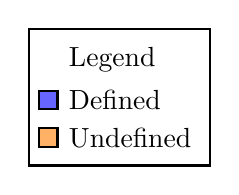
\begin{tikzpicture}
            \matrix [thick, draw=black] {
            \node[label=right:{Legend}] {}; \\
            \node[thick, shape=rectangle, draw=black, fill=blue!60,   label=right:{Defined}](0) {}; \\
            \node[thick, shape=rectangle, draw=black, fill=orange!60, label=right:{Undefined}](1) {}; \\
            };
        \end{tikzpicture}
    \end{subfigure}
    \caption{Breakdown of how many test approaches are undefined.}
    \label{fig:undefPies}
\end{figure*}


\subsection{Missing Terms}\label{future-miss-terms}
\imptodo{Fill in}

\subsection{Detecting More Flaws}\label{future-detect-flaws}
\imptodo{Fill in}
